\def\QRCODE{tp_en_attente_TUT.IMG.tomography_pythonqrcode.png}
\def\QRPAGE{http://www.iptutorials.science/tree/master/tp_en_attente/TUT.IMG.tomography/python}
\pcorrectionsection{Python correction}

\begin{python}
import numpy as np
import matplotlib.pyplot as plt

from skimage.io import imread
from skimage.transform import radon, rescale, rotate
from scipy.signal import convolve
import skimage.io
\end{python}


\subsection{Acquisition simulation}
The phantom image is first loaded and displayed.

\begin{python}
# Read image
image = imread("phantom.png", as_gray=True)
image = image[:,:,0];
plt.imshow(image, cmap='gray');
\end{python}

The simulation of the projection is simply an addition of all gray-levels of the pixels, after rotating the image in order to simulate the rotation of the object (or of the sensor).
\iflabelexists{fig:tomography:enonce:contri}{See Fig.\ref{fig:tomography:enonce:contri}}{See Fig.\ref{fig:tomography:python:contri}.

\begin{figure}[htbp]
 \centering
 
\includegraphics[width=.4\linewidth]{contri.python.png}
 \caption{Simulation of the projection: contribution of a line $D$ before rotation.}
 \label{fig:tomography:python:contri}
\end{figure}
}

\begin{python}
def simuProjection(I, theta):
    """
    simulation of the generation of a sinogram
    I : original image (phantom for example)
    theta: angles of projection
    """
    N = I.shape[1];
    M = len(theta);
    S = np.zeros((N,M));

    for i,ang in enumerate(theta):
        image1 = rotate(I, ang);
        S[:,i] = np.sum(image1, axis=1);
        
    return S;
\end{python}


\subsection{Backprojection algorithm}
The backprojection algorithm will sum-up all the contributions of each projection.

\begin{python}
def backprojection(P, theta, filtre):
    """
    Backprojection of
    P: image
    theta: list of projection angles
    filtre: bool, True if filtered
    """
    
    N = P.shape[0];
    R = np.zeros((N,N));
    
    # in case of filtered back-projection
    if filtre:
        h = RamLak(31);
    
    # loops over all angles
    for i,ang in enumerate(theta):
        proj = P[:,i];
        
        # filtered back-projection
        if filtre:
            proj = convolve(proj, h, mode='same');
        
        proj2 = np.matlib.repmat(proj, N, 1);
        proj2 = rotate(proj2, ang);
        R = R + proj2;
    return R.transpose();
\end{python}

The results is better in the case of a filtered backprojection. The RamLak function is provided and illustrated in Fig.\ref{fig:tomography:python:ramlak}.
\begin{python}
def RamLak(width):
    """
    Ramlak filter of size width
    width must be odd
    """
    ramlak = np.zeros((2*width+1,));
    for indice, val in enumerate(np.arange(-width, width+1)):
      val = np.abs(val);

      if val==0: # center
         ramlak[indice]=np.pi/4;
      else:
        if val%2==1: # even indices
            ramlak[indice]=-1/(np.pi*val**2);
        else: # odd indices
            ramlak[indice]=0;
    
    return ramlak;
\end{python}

\begin{figure}[htbp]
 \centering
 
 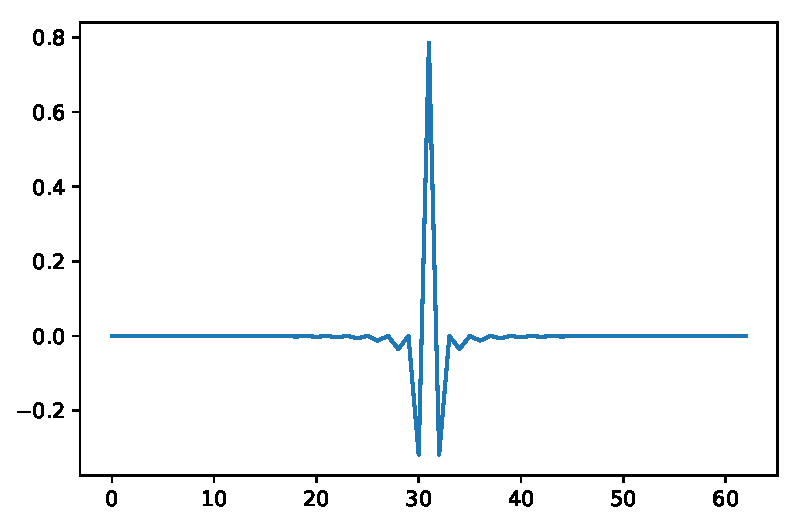
\includegraphics[width=.45\linewidth]{ramlak.pdf}
 
 \caption{RamLak function.}
 \label{fig:tomography:python:ramlak}
\end{figure}

The reconstruction of the original image is obtained by the following code:
\begin{python}
# Performs unfiltered backprojection
ubp = backprojection(P, theta, False);
plt.figure();
plt.imshow(ubp, cmap='gray');
plt.show()

# Performs filtered backprojection
fbp = backprojection(P, theta, True);
plt.figure();
plt.imshow(fbp, cmap='gray');
plt.show()
\end{python}

\begin{figure}[htbp]
 \centering
 
 \subfloat[Original phantom image.]{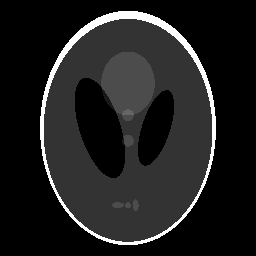
\includegraphics[width=.3\linewidth]{phantom.png}}\hfill
  \subfloat[Unfiltered backprojection.]{
\includegraphics[width=.3\linewidth]{unfiltered_backprojection.python.png}}\hfill
 \subfloat[Filtered backprojection.]{
\includegraphics[width=.3\linewidth]{filtered_backprojection.python.png}}
 \caption{Reconstruction by backprojection.}
 \label{fig:tomography:python:backprojection}
\end{figure}

